\documentclass[10pt]{beamer}

% %%% Style %%%
\mode<presentation>
{
  \usetheme{Berlin}
  \setbeamertemplate{blocks}[rounded]
  \setbeamercolor{block title}{bg=gray}
  \setbeamercovered{transparent}
}

% %%% Packages %%%
% Babel and fonts
\usepackage[english]{babel}
\usepackage[utf8]{inputenc}

% Graphics and images
\usepackage{xcolor}
\usepackage{graphicx}
\DeclareGraphicsExtensions{.pdf,.png,.jpg, .eps}
\usepackage{relsize}
\usepackage{colortbl}


% Math notation and symbols
\usepackage{mathrsfs}
\usepackage{amsthm}
\usepackage{bbold}
\usepackage{amsfonts}
\usepackage{amsmath}
\usepackage{amssymb}
% \usepackage{algorithm}
\usepackage{algpseudocode}
\usepackage{listings}

% \DeclareMathOperator*{\len}{\text{length of }}
% Backup slides
\usepackage{appendixnumberbeamer}

% Tables, Colums and the like
\usepackage{longtable}
\usepackage{listings}

% Hyperref
\usepackage{hyperref} 

% Boxes
\usepackage{fancybox}
\usepackage{lmodern}
\usepackage{tikz}
\usepackage{tcolorbox}
\usepackage{mdframed}	

\usepackage{hyperref}
\usepackage{listings}
\usepackage{setspace}
\usepackage{subfiles}
\usepackage{alltt}
\usepackage{mathtools}
\usepackage{fancyvrb}
\usepackage{url}

\usepackage{tikz}
\usetikzlibrary{shapes,arrows,positioning,calc}

\usepackage{xparse}
\usepackage{ifthen}
\usepackage{twoopt}

% Custom packages (needs absolute path from root document
%  Usage: \usepackage{appendixnumberbeamer}
%  Custom title page

\makeatletter

\setbeamertemplate{footline}
{
  \leavevmode%
  \hbox{%
  \begin{beamercolorbox}[wd=0.25\paperwidth,ht=2.25ex,dp=1ex,center]{author in head/foot}%
    \usebeamerfont{author in head/foot}\insertshortauthor
  \end{beamercolorbox}%
  \begin{beamercolorbox}[wd=0.50\paperwidth,ht=2.25ex,dp=1ex,center]{title in head/foot}%
    \usebeamerfont{title in head/foot}\inserttitle
  \end{beamercolorbox}%
  \begin{beamercolorbox}[wd=0.25\paperwidth,ht=2.25ex,dp=1ex,right]{date in head/foot}%
    \insertframenumber{} / \inserttotalframenumber\hspace*{2ex} 
  \end{beamercolorbox}}%
  \vskip0pt%
}
\makeatother

\makeatletter
\setbeamertemplate{headline}
{
  \leavevmode%
  \hbox{%
  \begin{beamercolorbox}[wd=\paperwidth,ht=2.25ex,dp=1ex,center]{title in head/foot}%
  \end{beamercolorbox}%
  }%
  \vskip0pt%
}
\makeatother

\defbeamertemplate*{title page}{customized}[1][]
{
  \begin{center}
    \begin{variableblock}{}{}{bg=blue}
      \begin{center}
	\usebeamerfont{title}\inserttitle\par
      \end{center}
    \end{variableblock}
  \end{center}

  \begin{center}
    \begin{minipage}{1.0\textwidth}
      \begin{center}
	\insertauthor

	\begin{scriptsize}
	  \insertdate
	\end{scriptsize}

      \end{center}
    \end{minipage}
  \end{center}
}

% vim:ft=plaintex:
%
%  Written and (C) by J�r�me Lelong <jerome.lelong@gmail.com>
%  2007 - 2012
% 
%  This program is free software; you can redistribute it and/or modify it
%  under the terms of the GNU General Public License as published by the
%  Free Software Foundation; either version 3 of the License, or (at your
%  option) any later version.
% 
%  This program is distributed in the hope that it will be useful, but
%  WITHOUT ANY WARRANTY; without even the implied warranty of
%  MERCHANTABILITY or FITNESS FOR A PARTICULAR PURPOSE.  See the GNU
%  General Public License for more details.
% 
%  You should have received a copy of the GNU General Public License along
%  with this program.  If not, see <http://www.gnu.org/licenses/>. 
% 
%  This small piece of code fixes the frame numbering in beamer when using
%  an appendix such  that the slides of the appendix are not counted in the
%  total framenumber of the main part of the document. The total
%  framenumber counter is reset to 0 and starts counting again when
%  entering the appendix.
% 
%  Usage: \usepackage{appendixnumberbeamer}
%  and declare the appendix as usual using the \appendix command.


\makeatletter


\let\appendixtotalframenumber\empty
\def\mainend{-1}
\let\appendixorig\appendix

% Redefine the \appendix command:
%   - it resets the framenumber counter 
%   - freezes the total framenumber for this first part of the document
\def\appendix{
  \edef\mainend{\theframenumber}
  \immediate\write\@auxout{\string\global\string\@namedef{mainendframenumber}{\mainend}}
  \appendixorig
  \def\inserttotalframenumber{\appendixtotalframenumber}%
  \setcounter{framenumber}{0}
}

% To be called at the end of document to fix the total framenumber in the
% main document and in the appendix.
\def\pageatend{
  \edef\appendixend{\theframenumber}
  \ifnum\mainend>0%
  \immediate\write\@auxout{\string\global\string\@namedef{appendixtotalframenumber}{\appendixend}}%
  \immediate\write\@auxout{\string\global\string\@namedef{inserttotalframenumber}{\mainend}}%
  \immediate\write\@auxout{\string\@writefile{nav}{\noexpand \headcommand {%
        \noexpand \def\noexpand \inserttotalframenumber{\mainend}}}}%
  \immediate\write\@auxout{\string\@writefile{nav}{\noexpand \headcommand {%
        \noexpand \def\noexpand \appendixtotalframenumber{\appendixend}}}}%
  \else
  \fi
}


\AtEndDocument{\pageatend}
\makeatother


% %%% Macros and custom commands %%%
\DeclareMathOperator*{\len}{\textbf{length of }}

\newcommand{\btVFill}{\vskip0pt plus 1filll}

\setbeamercolor{structure}{fg=cyan!90!black}

\newenvironment{variableblock}[3]{%
\setbeamercolor{block body}{#2}
\setbeamercolor{block title}{#3}
\begin{block}{#1}}{\end{block}}

\lstdefinestyle{JavaPlain}{ %
basicstyle=\scriptsize\ttfamily, % the size of the fonts 
numbers=left,                   % where to put the line-numbers
numberstyle=\tiny,      % the size of the fonts that are used for th
stepnumber=1,                   % the step between two line-numbers
numbersep=5pt,                  % how far the line-numbers are from the code
backgroundcolor=\color{white},  % choose the background color
showspaces=false,               % show spaces adding particular underscores
showstringspaces=false,         % underline spaces within strings
showtabs=false,                 % show tabs within strings adding 
frame=single,           % adds a frame around the code
tabsize=2,          % sets default tabsize to 2 spaces
captionpos=b,           % sets the caption-position to bottom
breaklines=true,        % sets automatic line breaking
breakatwhitespace=false,    % sets if automatic breaks should only happen
fancyvrb=true,
fvcmdparams=textbf 1 textit 1,
}

% Colors
\definecolor{ballblue}{rgb}{0.13, 0.67, 0.8}
\definecolor{brown(web)}{rgb}{0.65, 0.16, 0.16}
\definecolor{brown(traditional)}{rgb}{0.59, 0.29, 0.0}

\newcommand\Red[1]{\textcolor{red}{#1}}
\newcommand\Green[1]{\textcolor{green!50!black}{#1}}
\newcommand\LightGreen[1]{\textcolor{green!60!black}{#1}}
\newcommand\Blue[1]{\textcolor{blue!60!white}{#1}}
\newcommand\Violet[1]{\textcolor{violet}{#1}}
\newcommand\LightBlue[1]{\textcolor{ballblue}{#1}}
\newcommand\Grey[1]{\textcolor{gray}{#1}}
\newcommand\Gray[1]{\textcolor{gray}{#1}}
\newcommand\Brown[1]{\textcolor{brown(web)}{#1}}
\newcommand\LightBrown[1]{\textcolor{brown(traditional)}{#1}}

% Helpers
\newcommand\Jcomment[1]{\LightGreen{// #1}}
\newcommand\JcommentMulti[1]{\LightGreen{/* #1}}
\newcommand\String[1]{\textcolor{blue!80!blue}{#1}}
\newcommand\Word[1]{\textcolor{purple!90!red}{#1}}
\newcommand\bang{!}
\newcommand\pipe{\|}

% Prints
% \newcommand\Jprintf[2][]{\LightBlue{printf}(\String{#1}, #2)}
\newcommandtwoopt{\Jprintf}[2][-NoValue-][-NoValue-]{%
    \ifthenelse{\equal{#2}{-NoValue-}}{\LightBlue{printf}(\String{#1})}{\LightBlue{printf}(\String{#1}, #2)}%
}

\newcommand\Jprintln[1]{\LightBlue{println}(\String{#1})}
\newcommand\JprintLN{\LightBlue{println}}

% Control structures
% Shortcut for JavaFor:
% \JavaFor (\Blue!init| \Green!n <= Math.sqrt(numero);| \Violet!n++|)
\newcommand\JavaForColors[3]{\Blue{#1}; \Green{#2}; \Violet{#3}}

\newcommand\Jfor[1][-NoValue-]{%
  \ifthenelse{\equal{#1}{-NoValue-}}{\Word{for}}{\JavaForO[#1]}%
}

\newcommandtwoopt{\JavaForO}[3][-NoValue-][-NoValue-]{%
    \JavaForOptions{#1}{#2}{#3}%
}

\DeclareDocumentCommand\JavaForOptions{ ggg }{%
  \Word{for}\IfValueT{#1}{%
    (\JavaForColors{#1}{#2}{#3}) %
  }%
}

% Shortcut for JavaFor:
% \JavaFor (\Blue!init| \Green!n <= Math.sqrt(numero);| \Violet!n++|)
\newcommand\Jif[1][-NoValue-]{%
  \ifthenelse{\equal{#1}{-NoValue-}}{\Word{if}}{\Word{if} (\Green{#1})}%
}

% Other reserved words
\newcommand\Jstatic{\Word{static}}
\newcommand\Jpublic{\Word{public}}
\newcommand\Jprivate{\Word{private}}
\newcommand\Jdouble{\Word{double}}
\newcommand\Jfloat{\Word{float}}
\newcommand\Jint{\Word{int}}
\newcommand\Jvoid{\Word{void}}
\newcommand\Jreturn{\Word{return}}
\newcommand\Jclass{\Word{class}}
\newcommand\Jargs{\LightBrown{args}}

\newenvironment{JavaCodePlain}[1][]
  { \VerbatimEnvironment%
    \begin{Verbatim}[#1]}
  { \end{Verbatim}  } 

\algdef{SE}[DOWHILE]{Do}{DoWhile}{\algorithmicdo}[1]{\algorithmicwhile\ #1}%
\renewcommand{\algorithmicrequire}{\textbf{Input:}}
\renewcommand{\algorithmicensure}{\textbf{Output:}}

\title[Laboratorio di Informatica - Lezione 4]{Laboratorio di Informatica \\ Lezione 4}
\author[Cristian Consonni]{Cristian Consonni}
\date[28/10/2015]{28 ottobre 2015}
\institute[UniTN]{Università degli Studi di Trento}

% %%% Put slides with section name at the begining of each section %%%
\AtBeginSection[]
{
  \begin{frame}<beamer>
    \frametitle{Outline for section \thesection}
    \tableofcontents[currentsection]
  \end{frame}
}
\setbeamertemplate{navigation symbols}{}

\begin{document}

%%%%%%%%%% TITLE %%%%%%%%%%
% Formerly part of title.tex
\begin{frame}
  \titlepage
\end{frame}

\begin{frame}{Outline}
  \tableofcontents
\end{frame}
%%%%%%%%%% END TITLE %%%%%%%%%%

\subsection[Informazioni generali]{Informazioni generali}

\begin{frame}{Chi sono}
  Cristian Consonni

  \begin{itemize}
    \item \textbf{DISI - Dipartimento di Ingegneria e Scienza dell'Informazione}
    \item \textbf{Pagina web} del laboratorio: \structure{\url{http://disi.unitn.it/~consonni/teaching}}
    \item \textbf{Email}: \structure{\url{cristian.consonni@unitn.it}}
    \item \textbf{Ufficio}: Povo 2 - Open Space 9
      \begin{itemize}
	\item Per domande: scrivetemi una mail
	\item Ricevimento: su appuntamento via mail
      \end{itemize}
  \end{itemize}
\end{frame}



\begin{frame}{Obiettivi del laboratorio}
  Obiettivi del laboratorio:
  \begin{itemize}
    \item Apprendere i fondamenti di un vero linguaggio di programmazione (Java)
    \item Svolgere il progetto
  \end{itemize}

  Obiettivi del laboratorio
  \begin{enumerate}
    \item Fare esperienza in laboratorio
    \item Raggiungere una buona manualità nell'uso degli strumenti standard
    \item Esercizi
  \end{enumerate}

\end{frame}

\pgfdeclareimage[width=0.6\paperwidth]{xkcd}{img/11th_grade.png}
\begin{frame}{Manualità (I)}
  \begin{center}
    \pgfuseimage{xkcd}
  \end{center}
  \url{https://xkcd.com/519/}
\end{frame}

\pgfdeclareimage[width=0.6\paperwidth]{abstrusegoose}{img/ars_longa_vita_brevis.png}
\begin{frame}{Manualità (II)}
  \textbf{How to Teach Yourself Programming:}\footnote{\url{http://abstrusegoose.com/249}}
  \begin{center}
    \pgfuseimage{abstrusegoose}
  \end{center}
  
\end{frame}

\begin{frame}{Slides}

  Info sulle slide:
  \begin{itemize}
    \item le slide del corso saranno rese disponibili sul sito;
    \item segnalate pure eventuali errori;
    \item cercherò di pubblicare le slide in anticipo rispetto alla lezione;
    \item queste slide sono prodotte con \LaTeX \; \texttt{Beamer} (\emph{usate} \LaTeX!);
  \end{itemize}

  Segnalazioni di materiale:
  \begin{itemize}
    \item Materiale da voi prodotto;
    \item Cose interessanti che trovate online;
    \item Possiamo valutare insieme se riutilizzarle;
  \end{itemize}
\end{frame}

\section{Canali standard}

\begin{frame}{Note sullo stile}

  \begin{itemize}
    \item Utilizzare il camelCase/PascalCase
    \begin{itemize}
      \item \scriptsize{\url{https://en.wikipedia.org/w/index.php?title=CamelCase&oldid=686054689}}
    \end{itemize}
    \item Quando create una classe, la prima lettera è \textbf{Maiuscola}, ad es. \texttt{TestPrimo};
    \item I metodi e le variabili hanno la lettera iniziale \textbf{minuscola}, ad es. \texttt{sommaInteri}, \texttt{stampaVettore};
    \item le costanti vanno indicate tutte in \textbf{MAIUSCOLO}, ad es. \texttt{NMAX}, \texttt{EPSILON};
  \end{itemize}

\end{frame}

\begin{frame}{Canali standard (I)}

  \begin{quote}
     «I \textbf{canali standard} (o \textbf{standard streams}), in tutti i moderni sistemi operativi,
     rappresentano i dispositivi logici di input e di output che collegano un programma 
     con l'ambiente operativo in cui esso viene eseguito (tipicamente un terminale testuale)
     e che sono connessi automaticamente al suo avvio.»
  \end{quote}

  \vfill

  \begin{minipage}[c]{10cm}
    \scriptsize{fonte: \url{https://it.wikipedia.org/wiki/Canali_standard}}
  \end{minipage}

\end{frame}

\begin{frame}{Canali standard (II)}

  Esistono tre canali standard predifiniti:
  \begin{itemize}
   \item \texttt{\textbf{stdin}}: \emph{standard input};
   \item \texttt{\textbf{stdout}}: \emph{standard output};
   \item \texttt{\textbf{stderr}}: \emph{standard error};
  \end{itemize}

\end{frame}

\begin{frame}[fragile]\frametitle{Canali standard (III)}

  I canali standard possono essere rappresentati nel modo seguente:
  \begin{center}
    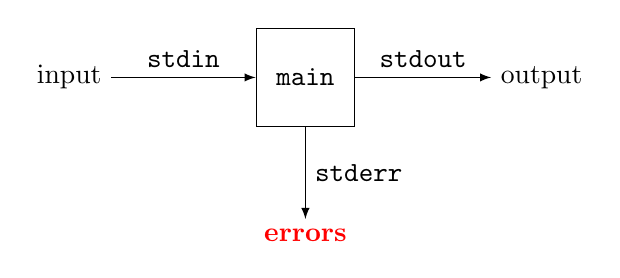
\begin{tikzpicture}[baseline=-0.5ex, on grid, node distance=2cm]
      \node (input) {input};
      \node[draw,right= 3cm of input, minimum size=1.25cm] (prog) {\texttt{main}}; 
      \node[right= 3cm of prog] (output) {output};
      \node[below= 2cm of prog] (error) {\Red{\textbf{errors}}};

      \draw[-latex] (input) -- node[anchor=south,pos=0.5]{\texttt{stdin}}(prog);
      \draw[-latex] (prog)  -- node[anchor=south,pos=0.5]{\texttt{stdout}}(output);
      \draw[-latex] (prog)  -- node[anchor=west,pos=0.5]{\texttt{stderr}}(error);
    \end{tikzpicture}
  \end{center}

\end{frame}

\begin{frame}{Canali standard (IV)}
  Questi canali sono tutti legati al \textbf{terminale} (o \emph{console} o \emph{command prompt}).
  
  \pause{Per esempio, tramite il terminale possiamo:}
  \begin{itemize}[<+(1)->]
   \item leggere un input da terminale (\texttt{stdin});
   \item stamparlo a schermo (\texttt{stdout});
   \item raccogliere un messaggio di errore (\texttt{stderr});
  \end{itemize}
\end{frame} 

\begin{frame}{Canali standard (V)}

  In sistemi Unix (Linux e Mac OS X) è possibile separare (redirezionare) i diversi streams
  lanciando il comando con una sintassi speciale:
  \begin{center}
    \texttt{java LetturaFile <in 1>out 2>err}
  \end{center}
  
   \begin{itemize}[<+(1)->]
     \item \texttt{<} redireziona lo \texttt{stdin};
     \item \texttt{1>} redireziona lo \texttt{stdout};
     \item \texttt{2>} redireziona lo \texttt{stderr};
   \end{itemize}

\end{frame}


\section{Input da tastiera}

\begin{frame}[fragile]\frametitle{Lettura input da tastiera (I)}

  Abbiamo già visto che per stampare dei valori a schermo si usa:
  \begin{itemize}
    \item \texttt{\textbf{System.out}}
  \end{itemize}
  questo permette di interagire con lo \texttt{stdout}.
  
  ${}$

  Analogamente:
  \begin{itemize}
    \item \texttt{\textbf{System.in}}
  \end{itemize}
  permette di interagire con lo \texttt{stdin}.
  
%   ${}$
% 
%   Nella libreria \texttt{java.util} di Java esiste l'oggetto \texttt{\textbf{Scanner}} 
%   che ci permette di utilizzare l’input della console:
%   \begin{JavaCodePlain}[commandchars=\\!|]
%   Scanner input = new Scanner(System.in);
%   \end{JavaCodePlain}     

\end{frame}

\begin{frame}[fragile]\frametitle{Lettura input da tastiera (II)}
  Nella libreria \texttt{java.util} di Java esiste l'oggetto \texttt{\textbf{Scanner}} 
  che ci permette di utilizzare l’input della console:
  
  \begin{JavaCodePlain}[commandchars=\\!|]
  \Jimport java.util.Scanner;

  \Jpublic \Jclass LetturaFile {

    \Jpublic \Jstatic \Jvoid main(String[] \Jargs) {
      Scanner input = \Jnew Scanner(\JsystemIn);
    
      \dots
      
      \Jcomment!Al termine della lettura chiudere il canale di input|
      input.close();
    }
  }
  \end{JavaCodePlain}     

\end{frame}

\begin{frame}[fragile]\frametitle{Lettura input da tastiera (III)}
  
  Per potere utilizzare \texttt{\textbf{Scanner}} dobbiamo \emph{importare}
  la libreria \texttt{\textbf{java.util}} aggiungendo la riga:
  \begin{JavaCodePlain}[commandchars=\\!|]
  \Jimport java.util.Scanner;
  \end{JavaCodePlain}
  all'inizio del file.
  
  ${}$

  Lo statement \Word{import} è il modo in cui si possono \emph{importare} librerie in
  un programma Java.

  ${}$

  Una libreria è un insieme di funzioni e/o strutture dati predefinite e predisposte
  per essere riutilizzate facilmente all'interno di svariati programmi.

\end{frame}

\begin{frame}[fragile]\frametitle{Modalità di lettura da \texttt{stdin} (I)}

  Dopo aver dichiarato l'oggetto di tipo \texttt{Scanner}
  \begin{JavaCodePlain}[commandchars=\\!|]
  Scanner input = \Jnew Scanner(\JsystemIn);
  \end{JavaCodePlain}

  si possono usare i seguenti \textbf{metodi}:
  \begin{itemize}
   \item \texttt{input.nextInt()} \structure{$\Rightarrow$} lettura di un \Jint;
   \item \texttt{input.nextDouble()} \structure{$\Rightarrow$} lettura di un \Jdouble;
   \item \texttt{input.next()} \structure{$\Rightarrow$} lettura di una stringa;
   \item \texttt{input.nextLine()} \structure{$\Rightarrow$} legge l'intera linea fino al
	 carattere \texttt{newline} (Invio);
  \end{itemize}

\end{frame}

\begin{frame}[fragile]\frametitle{Modalità di lettura da \texttt{stdin} (II)}

  Se viene inserito un valore di un tipo non corrispondendente viene causato
  un \textbf{errore} ovvero viene \emph{lanciata un'\textbf{eccezione}}.

  ${}$\\
  
  \pause{
  Se per esempio uso \textbf{\texttt{input.nextInt()}}:
  \begin{JavaCodePlain}[commandchars=\\!|]
  Inserisci un numero intero: \Green!3.2|
  \end{JavaCodePlain}

  \begin{redtext}
  \begin{JavaCodePlain}[commandchars=\\!|]
  \textbf!Exception| in thread "main" java.util.InputMismatchException
    at java.util.Scanner.throwFor(Scanner.java:864)
    at java.util.Scanner.next(Scanner.java:1485)
    at java.util.Scanner.nextInt(Scanner.java:2117)
    at java.util.Scanner.nextInt(Scanner.java:2076)
    at LetturaIntero.main(LetturaIntero.java:11)
  \end{JavaCodePlain}
  \end{redtext}
  }

\end{frame}

\begin{frame}[fragile]\frametitle{Modalità di lettura da \texttt{stdin} (III)}

  Esistono dei metodi per controllare il tipo di dato inserito:
  \begin{itemize}
   \item \texttt{input.hasNextInt()} \structure{$\Rightarrow$} controlla che venga letto un \Jint;
   \item \texttt{input.hasNextDouble()} \structure{$\Rightarrow$} controlla che venga letto un \Jdouble;
   \item etc.
  \end{itemize}

  Queste funzioni ritornano \Word{true} se il prossimo valore è del tipo indicato:
  \begin{JavaCodePlain}[commandchars=\\!|]
    \Jprint!"Inserisci la tua altezza (in cm): "|;
    \Jwhile (\bang!|input.hasNextInt()) {
      \Jprintln!"Il numero inserito non è un intero valido."|;
      \Jprint!"Inserisci la tua altezza (in cm): "|;
      input.next();
    }   
  \end{JavaCodePlain}


\end{frame}



\section{Output}

\begin{frame}{Scrittura su \texttt{stdout} (I)}
  Abbiamo già visto dei comandi/funzioni per scrivere sullo standard output (``a schermo''):
  \begin{itemize}
   \item \texttt{System.out.\LightBlue{print}( \String{stringa} )}
   \item \texttt{System.out.\LightBlue{prinlnf}( \String{stringa} )}
   \item \texttt{System.out.\LightBlue{printf}( \String{formato}, argomenti, \dots)}
  \end{itemize}
 
\end{frame}

\begin{frame}{Scrittura su \texttt{stdout} (II)}

Alcune cose utili:
  \begin{itemize}
   \item Con \LightBlue{printf} il formato \String{"\%nd"}, dove $n$ è un numero (intero),
   stampa spazi aggiuntivi in modo tale che il numero occupi sempre $n$ spazi (si veda 
   l'esercizio \texttt{MatriceTrasposta});
   \item Con \LightBlue{printf} il formato \String{"\%0nd"}, dove $n$ è un numero (intero),
   stampa degli zeri aggiuntivi in modo tale che il numero occupi sempre $n$ spazi, ad
   esempio \String{"\%03d"} stampa il numero \texttt{7} come \texttt{007};
   \item altre \emph{sequenze di escape} particolari sono \texttt{\string\t} per inserire una
   tabulazione (un numero di spazi variabile che allinea l'output lungo una data colonna)
  \end{itemize}
\end{frame}


\section{Esercizi (parte I)}
\begin{frame}{Esercizi (parte I)}

  \begin{enumerate}
    \item Scrivere una funzione testa se un numero intero è primo (restituendo un booleano);
    \item Scrivere una procedura che stampi una parola (o una frase)
    al contrario. Ad esempio:
    \begin{itemize}
      \item ``gatto'' $\rightarrow$ ottag;
      \item ``anna'' $\rightarrow$ anna;
    \end{itemize}
    \item scrivere una funzione che calcoli la somma dei numeri interi da 1 a N;
    \item riscrivere la funzione precedente in modo ricorsivo;
  \end{enumerate}
\end{frame}


\section{Lettura da File}

\begin{frame}{Lettura da file (I)}

  Il caso della lettura da file è simile a quello della lettura da \texttt{stdin}:
  \begin{itemize}
   \item viene creato un \textbf{oggetto} \texttt{File} che rappresenta il file nel
   \emph{filesystem}.
   \item si usa uno \texttt{Scanner} come nel caso della lettura da \emph{standard input}
  \end{itemize}

\end{frame}

\begin{frame}[fragile]\frametitle{Lettura da file (II)}

  \begin{JavaCodePlain}[commandchars=\\!|]
  \Jimport java.io.File;
  \Jimport java.util.Scanner;

  \Jpublic \Jclass LetturaFile {
    \Jpublic \Jstatic \Jvoid main(String[] \Jargs) {

      File file = \Jnew File(\String!"esempio.txt"|);
      Scanner scan = \Jnew Scanner(file);

      \dots
  \end{JavaCodePlain}

  \pause{
  Si noti l'utilizzo delle due librerie:
  \begin{itemize}
   \item \texttt{java.io.File}
   \item \texttt{java.util.Scanner}
  \end{itemize}
  }
  
\end{frame}

\begin{frame}{Percorsi (I)}
  Prima abbiamo indicato \String{"esempio.txt"} come nome del file, in generale possiamo
  indicare un \textbf{percorso} (o \textbf{path}).

  ${}$\\

  I percorsi si specificano in modo diverso per sistemi operativi diversi:
  \begin{itemize}
   \item \structure{Unix (Linux, Mac OS X)} \\
	 \texttt{\Red{\textbf{/}}utente\Red{\textbf{/}}unitn\Red{\textbf{/}}informatica\Red{\textbf{/}}lab\Red{\textbf{/}}prova.txt}
   \item \structure{Windows} \\
	  \texttt{C:\Red{\textbf{$\backslash$}}utente\Red{\textbf{$\backslash$}}unitn\Red{\textbf{$\backslash$}}informatica\Red{\textbf{$\backslash$}}lab\Red{\textbf{$\backslash$}}prova.txt}
  \end{itemize}
  
  Il nome del file va sempre inserito \textbf{completo di estensione}.
  
\end{frame}

\begin{frame}{Percorsi (II)}
  Inoltre un percorso può essere:
  \begin{itemize}
   \item \alert{relativo}, se si riferisce alla cartella corrente.
   \begin{itemize}
     \item i path relatvi si riferiscono alla cartella corrente (indicata con \texttt{.},
	   \texttt{..} alla cartella genitore di quella corrente).
     \item in Eclipse la cartella corrente è la \textbf{cartella principale del progetto} all'interno
     del \emph{workspace}.
     \item \String{"esempio.txt"} è un path relativo alla cartella corrente.
   \end{itemize}
   \item \alert{assoluto}, se si riferisce alla radice del filesystem
   (\texttt{\Red{\textbf{/}}} su sistemi Unix, \texttt{\Red{\textbf{C:$\backslash$}}} su Windows)
   \begin{itemize}
     \item \texttt{\Red{\textbf{/}}utente\Red{\textbf{/}}unitn\Red{\textbf{/}}info\Red{\textbf{/}}prova.txt}
     \item \texttt{\Red{\textbf{C:$\backslash$}}utente\Red{\textbf{$\backslash$}}unitn\Red{\textbf{$\backslash$}}info\Red{\textbf{$\backslash$}}prova.txt}
   \end{itemize}
  \end{itemize}

\end{frame}

\begin{frame}[fragile]\frametitle{Lettura da file (III)}

  \begin{JavaCodePlain}[commandchars=\\!|]
  \Jimport java.io.File;
  \Jimport java.util.Scanner;

  \Jpublic \Jclass LetturaFile {
    \Jpublic \Jstatic \Jvoid main(String[] \Jargs) {

      File file = \Jnew File(\String!"esempio.txt"|);
      Scanner \Yellow!scan| = \Red!new Scanner(file);|

      \dots
  \end{JavaCodePlain}

  Dopo aver scritto la dichiarazione dello \texttt{Scanner} dovremmo avere ottenuto:
  \begin{itemize}
   \item un \Yellow{warning} relativo al fatto che non chiudiamo lo scanner.
   \item un \Red{errore} relativo al fatto che una \textbf{eccezione non \`e gestita} (\emph{unhandled}).
  \end{itemize}

  
\end{frame}

\begin{frame}[fragile]\frametitle{Lettura da file (III)}

  \begin{JavaCodePlain}[commandchars=\\!|]
      Scanner scan = \Red!new Scanner(file);|
  \end{JavaCodePlain}

  Possiamo risolvere il problema in due modi (vedere anche la funzionalità
  \emph{quickfix} attivata con il comando \texttt{Ctrl + 1}):
  \begin{itemize}
   \item \textbf{lanciare} (\textbf{throw}) un'eccezione;
   \item \textbf{gestire} l'eccezione con il costrutto \textbf{\texttt{try - catch}};
  \end{itemize}

  Questo avviene perché la lettura da file può causare errori come per esempio un \emph{file non esistente}
  oppure \emph{non accessibile}.

\end{frame}

\begin{frame}[fragile]\frametitle{Lanciare un'eccezione}

  Se decidiamo di lanciare un'eccezione allora la dichiarazione del \texttt{main}
  viene modificata come segue:
  \begin{JavaCodePlain}[commandchars=\\!|]
  \Jimport java.io.File;
  \Jimport java.io.FileNotFoundException;
  \Jimport java.util.Scanner;

  \Jpublic \Jclass LetturaFile {

    \Word!\dots| main(String[] \Jargs) \Jthrows FileNotFoundException {
	  
      File file = \Jnew File(\String!"esempio.txt"|);
      Scanner scan = \Jnew Scanner(file);
      \dots
  \end{JavaCodePlain}

  Questa sintassi segnala che la funzione \texttt{main} può terminare a causa
  dell'errore \texttt{FileNotFoundException}.
																																
\end{frame}

\begin{frame}[fragile]\frametitle{Gestire un'eccezione con \texttt{try - catch}}

  La gestione dell'eccezione con \texttt{try - catch} avviene nel modo seguente:
  \begin{JavaCodePlain}[commandchars=\\!|]
  \Jimport java.io.File;
  \Jimport java.io.FileNotFoundException;
  \Jimport java.util.Scanner;

  \Jpublic \Jclass LetturaFile {

    \Jpublic \Jstatic \Jvoid main(String[] args) {
	    
      File file = new File(\String!"esempio.txt"|);
      Scanner scan;
      \Jtry {
        scan = new Scanner(file);
      } \Jcatch (FileNotFoundException e) {
        e.printStackTrace();
        \Jreturn;
      }
  
  \end{JavaCodePlain}

\end{frame}

\begin{frame}[fragile]\frametitle{Gestire un'eccezione con \texttt{try - catch} (II)}

  Le istruzioni nel blocco \texttt{try} vengono provate, se non causano errori l'esecuzione
  del programma prosegue normalmente, \textbf{in caso di errore} viene eseguito il blocco
  \texttt{catch}:
  \begin{JavaCodePlain}[commandchars=\\!|]
      \Jtry {
        scan = new Scanner(file);
      } \Jcatch (FileNotFoundException e) {
        \Jcomment!Queste istruzioni vengono eseguite solo se il|
        \Jcomment!blocco try ha restituito un errore del tipo|
        \Jcomment!FileNotFoundException|
        e.printStackTrace();
        \Jreturn;
      }  
  \end{JavaCodePlain}
  
  Lo scopo del blocco \texttt{try - catch} è quello di compiere le operazioni necessarie
  in conseguenza dell'errore.
\end{frame}


\section{Scrittura su File}

\begin{frame}{Scrittura file (I)}
  In modo analogo a quanto avviene per la lettura da file, per la scrittura:
  \begin{enumerate}[<+->]
   \item dobbiamo creare un oggetto che rappresenti il file su cui vogliamo scrivere,
   esso rappresenta il file nel \emph{filesystem};
   \item utilizziamo la classe di Java \alert{\texttt{FileWriter}} , questa classe si
   preoccupa di preparare il file per la scrittura gestendo, per esempio, l'\textbf{encoding} del file.
   \item creiamo un ``buffer'' \alert{\texttt{BufferedWriter}} che effettivamente conterrà il 
   testo da scrivere sul file.
   \item per scrivere usiamo il metodo \alert{\texttt{write()}} del buffer
   \item Quando abbiamo terminato, chiudiamo il buffer.
  \end{enumerate}
  
\end{frame}

\begin{frame}[fragile]\frametitle{Scrittura file (II)}

  \begin{JavaCodePlain}[commandchars=\\!|]
  \Jimport java.io.BufferedWriter;
  \Jimport java.io.File;
  \Jimport java.io.FileWriter;
  \Jimport java.io.IOException;

  \Jpublic \Jclass ScritturaFile {
    \Jpublic \Jstatic \Jvoid main(String[] args) throws IOException {

      String text = \String!"TestoEsempio"|;

      File file = \Jnew File(\String!"esempio.txt"|);
      FileWriter fw = \Jnew FileWriter(file);
      BufferedWriter bw = \Jnew BufferedWriter(fw);

      bw.write(text);
      bw.flush();
      bw.close();
      \dots
  \end{JavaCodePlain}
\end{frame}

\begin{frame}[fragile]\frametitle{Scrittura file (III)}

  Ogni qual volta aggiungiamo una delle classi necessarie alla scrittura
  su File Java segnala un errore che può essere risolto aggiungengo
  gli \Word{import} \emph{statement} necessari.

  \begin{JavaCodePlain}[commandchars=\\!|]
  \Jimport java.io.BufferedWriter;
  \Jimport java.io.File;
  \Jimport java.io.FileWriter;
  \Jimport java.io.IOException;
  \end{JavaCodePlain}
\end{frame}

\begin{frame}[fragile]\frametitle{Scrittura file (V)}

  Anche quando aggiungiamo il \texttt{FileWriter} dobbiamo preparci a gestire
  l'eccezione, in questo caso segnaliamo il fatto che il main può generare
  una \texttt{IOException}.

  \begin{JavaCodePlain}[commandchars=\\!|]

  \Jpublic \Jclass ScritturaFile {

    \Jpublic \Jstatic \Jvoid main(String[] args) \textbf!\Jthrows IOException| {

      String text = \String!"TestoEsempio"|;

      File file = \Jnew File(\String!"esempio.txt"|);
      FileWriter fw = \Jnew FileWriter(file);
      BufferedWriter bw = \Jnew BufferedWriter(fw);

  \end{JavaCodePlain}
\end{frame}

\begin{frame}[fragile]\frametitle{Scrittura file (VI)}

  \begin{JavaCodePlain}[commandchars=\\!|]

  \Jpublic \Jclass ScritturaFile {

    \Jpublic \Jstatic \Jvoid main(String[] args) \Jthrows IOException {

      String text = \String!"TestoEsempio"|;

      File file = \Jnew File(\String!"esempio.txt"|);
      FileWriter fw = \Jnew FileWriter(file);
      BufferedWriter bw = \Jnew BufferedWriter(fw);

      bw.write(text);
      \Jcomment!Forza lo svuotamento del buffer e la scrittura su|
      \Jcomment!file|
      bw.flush();
      bw.close();
    }
  }
  \end{JavaCodePlain}
\end{frame}


\section{Esercizi}
\subsection[Esercizi]{Esercizi}

\begin{frame}{Esercizi (I)}
  \begin{itemize}
   \item Scrivete un programma che stampi la canzone popolare inglese ``\emph{99 bottiglie di birra}''
   \item (vedete anche \url{https://esolangs.org/wiki/99_bottles_of_beer})
  \end{itemize}
  \begin{quote}
   «99 bottles of beer on the wall, 99 bottles of beer.\newline
   Take one down, pass it around, 98 bottles of beer on the wall \newline
   99 bottles of beer on the wall, 99 bottles of beer.\newline
   Take one down, pass it around, 98 bottles of beer on the wall  \newline
   ...\newline
   1 bottle of beer on the wall, 1 bottle of beer.\newline
   Take one down, pass it around, no more bottles of beer on the wall\newline
   There no more bottles of beer on the wall, no more bottles of beer.»
  \end{quote}

\end{frame}

\begin{frame}{Esercizi (II)}
  \begin{itemize}
    \item Utilizzando il ciclo \texttt{while} scrivete un programma che dato un 
    intero stampi a schermo la ``tabellina''.
    Ad esempio, se il numero è 7 dovrete stampare a schermo:
    \begin{itemize}
      \item 7*0 = 0
      \item 7*1 = 7
      \item 7*2 = 14
      \item $\dots$
      \item 7*10 = 70
    \end{itemize}
    \item riscrivete il programma precendente usando il ciclo \texttt{for}.
  \end{itemize}
\end{frame}


\begin{frame}{Esercizi (III)}
  \begin{itemize}
   \item Scrivete un programma che calcoli il fattoriale di un numero intero a vostra scelta.
  \end{itemize}

  La definizione del fattoriale è la seguente:
  \begin{equation}
    n! = n \times (n - 1) \times \dots \times 1
  \end{equation}
  quindi il calcolo del fattoriale può essere definito da: 
  \begin{center}
    \begin{minipage}{8cm}
      \begin{algorithmic}[1]
	\State $fatt \gets ?$ \Comment Quale valore va messo qui?
	\For{$i \gets 1$ to $N$}
	  \State $fatt \gets fatt \times i$ 
	\EndFor
      \end{algorithmic}
   \end{minipage}
  \end{center}

\end{frame}

\begin{frame}{Esercizi (IV)}
  \begin{itemize}
    \item Scrivere un programma che stampi i valori della serie di Fibonacci minori di 10000.
    La serie di Fibonacci \`e definita da:
    \begin{equation*}
      \left\{\begin{aligned}
	  & x_0 = 1\\
	  & x_1 = 1\\
	  & x_{n+1} = x_{n} + x_{n-1}
      \end{aligned}\right.
    \end{equation*}
  \end{itemize}

\end{frame}


\begin{frame}{Esercizi (V)}
  \begin{itemize}
    \item Scrivere un programma che usi il metodo per il calcolo della radice quadrata di Newton.
    
    \begin{equation*}
      \left\{\begin{aligned}
	  & x_0 = 0.5\\
	  & x_{n +1} = 0.5 \cdot {x_n} (3  - zx^2_n)
      \end{aligned}\right.
    \end{equation*}
    \begin{equation*}
     \lim_{n \to \infty} x_{n} = \sqrt{z}
    \end{equation*}
  \end{itemize}
  
  Il programma deve calcolare la serie definita sopra fino a che l'errore $\varepsilon_{n} = |x^{2}_{n} - z|$,
  non è più piccolo di $10^{-3}$. Per il valore assoluto utilizzate la funzione \texttt{Math.\Blue{abs()}}.

\end{frame}

\begin{frame}{Esercizi (VI)}
  \begin{itemize}
    \item Metodo della bisezione
  \end{itemize}
  \begin{tiny}
    \url{https://ece.uwaterloo.ca/~dwharder/NumericalAnalysis/10RootFinding/bisection/bisection.gif}
  \end{tiny}

  \begin{scriptsize}
    \begin{center}
      \begin{minipage}{8cm}
	\begin{algorithmic}[1]
	  \Require Function $f$, endpoint values $a, b$, tolerance $\varepsilon$, maximum iterations $N_{MAX}$
		   $a < b$, either $f(a) < 0$ and $f(b) > 0$ or $f(a) > 0$ and $f(b) < 0$
	  \Ensure value which differs from $a$ root of $f(x)=0$ by less than $\varepsilon$
    
	  \State $N \gets 1$
	  \While{$N \leq N_{MAX}$}
	    \State $c \gets (a + b)/2$
	    \If{$f(c) = 0 \lor (b – a)/2 < \varepsilon$}
	      \State \texttt{\textbf{print}}(c)
	      \State \Return;
	    \EndIf
	    \State $N \gets N + 1$
	    \If{$sign(f(c)) = sign(f(a))$}
	      \State $a \gets c$
	    \Else 
	      \State $b \gets c$
	    \EndIf
	  \EndWhile
	  \State \texttt{\textbf{print}}(Non ho trovato risultati)
	\end{algorithmic}
      \end{minipage}
    \end{center}
  \end{scriptsize}

\end{frame}

\begin{frame}{Esercizi (VII)}
  Test di primalità
  \begin{itemize}
    \item Scrivere un programma che, dato un intero positivo, verifichi se quel numero è primo oppure no.
  \end{itemize}

   Un numero $n \in \mathbb{N}, n > 1$ \`e \textbf{primo} se e solo se \`e divisibile solo per $1$ e per
   se stesso.
\end{frame}

% \appendix
% \section*{Backup}
% \begin{frame}
\begin{Huge}
Backup 
\end{Huge}
\end{frame}


\end{document}
